\subsection{Obstacles}\label{s:staticObstacles}
 
\paragraph{Summary:} There is a need to asses filtered LiDAR readings into detected obstacle rating associated to each cell. There are known obstacles in the form of a map which are verified taking into the account visibility constraints.
    
\paragraph{Introduction:} The \emph{static obstacles} were used in the original concept \cite{gomola2017probabilistic}, the \emph{Avoidance Grid} and \emph{Movement Automaton} were repurposed to enable \emph{finite time deterministic} avoidance. A \emph{Constraint-based path search} and \emph{obstacle modeling} is summarized in \cite{hentenryck2009constraint}.

This section is handling basic problems of \emph{static obstacle} detection and its focused on following real-world fixed position threats:
\begin{enumerate}
    \item \emph{Static Obstacles} - detected by LiDAR sensor or fused from \emph{Obstacle Map} information source.
    
    \item \emph{Geo-fencing Areas} - defined by offline/online information source as permanent flight restriction zones. There is usually no physical obstacle. Space is considered as a \emph{hard/soft constraint}.
    
    \item \emph{Long-term bad weather Areas} - the \emph{weather} is often changing (hour period), there are \emph{weather events}  which last for \emph{hours} or \emph{days}.
\end{enumerate}


\paragraph{Changing Scanning Density of LiDAR:} A LiDAR sensor is scanning in conic section given by $distance Range$, $horizontal Range$, $vertical Range$, where distance range is in the interval $[0,maxDistance]$, horizontal offset range is in $[-\pi,\pi]$, and vertical offset range is in $[\varphi_s, \varphi_e]$.  

Let say that $\text{d} horizontal^\circ, \text{d} vertical^\circ$ is unitary angle offset in which one LiDAR send and return is executed. That means the \emph{LiDAR} ray is sent every $\text{d} horizontal^\circ, \text{d} vertical^\circ$ offset movement. The \emph{LiDAR} ray density is decreasing with \emph{distance offset}. The same amount of \emph{LiDAR} rays passes through $cell_{i,j,k}$ in Avoidance Grid.

A surface of the area given by some distance d and unitary offsets$\partial horizontal^\circ, \text{d} vertical^\circ$  is changing with $distance$. The minimal triggering area of the object surface is not changing. This fact has an impact on the count of the hits on the object surface. 

The example is given in (fig. \ref{fig:P01CountOfLiDARHits}) where we have two identical objects (red circle) in distances 5 and 10 meters. The closer object consumes 5 LiDAR beam hits, and the farther object consumes only 3 LiDAR beam hits. The probability of obstacle encounter is remaining the same for the closer and farther object. The \emph{detected obstacle rate} assessment should return the same  detected obstacle collision rate for objects with the same scanned surface (with different LiDAR ray hit count).

\begin{figure}[H]
    \centering
    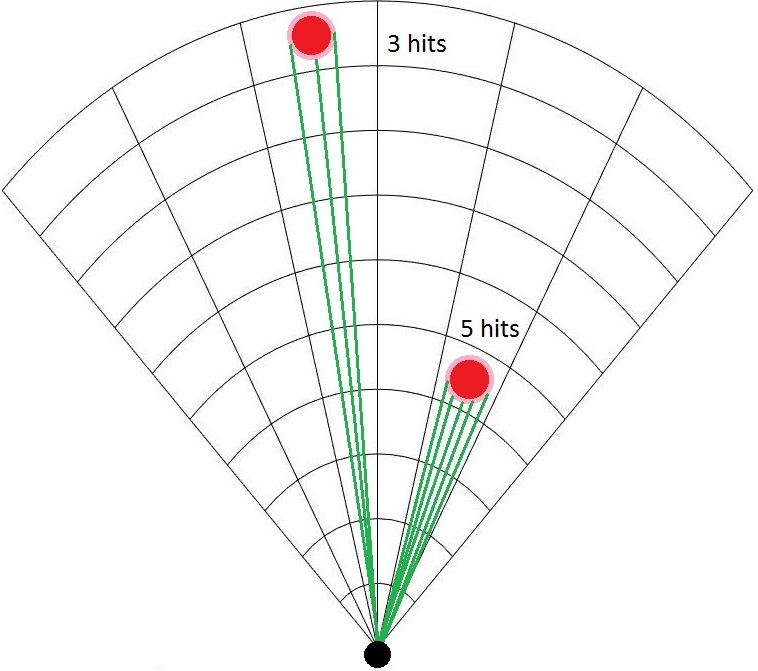
\includegraphics[width=0.7\textwidth]{\FIGDIR/TE051CountOfLiDARHits}
    \caption{Different count of LiDAR hits with different distance from UAS.}
    \label{fig:P01CountOfLiDARHits}
\end{figure}


\paragraph{Map and Detected Obstacles Fusion:} The concept of \emph{offline/online obstacle map} is mandatory in modern obstacle avoidance systems and increases the safety of navigation/avoidance path. The \emph{older} concept was considering only LiDAR reading or \emph{real-time sensor readings} in general \cite{gomola2017probabilistic}. 

\begin{figure}[htbp]
    \centering
    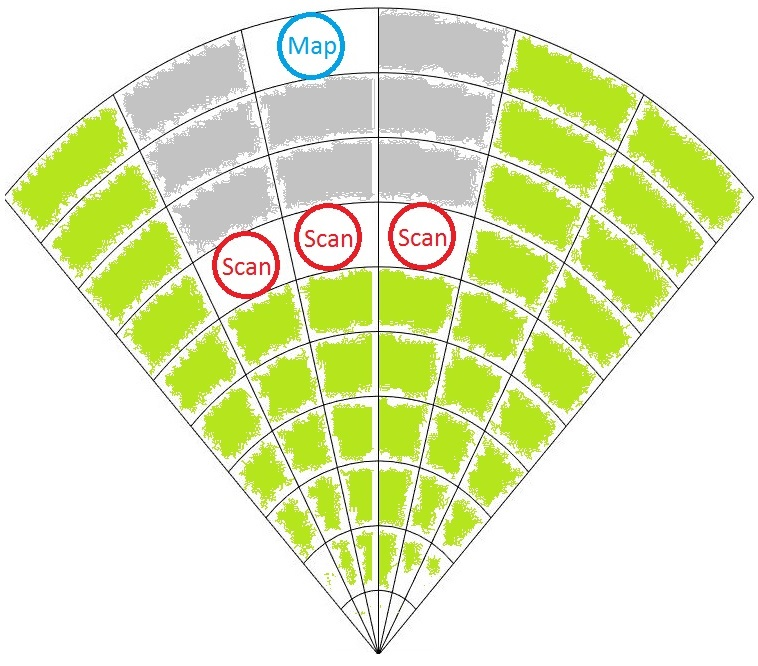
\includegraphics[width=0.7\textwidth]{\FIGDIR/TE053OvershadowedMapobstacle}
    \caption{Overshadowed map obstacle by detected obstacles.}
    \label{fig:P02OvershadowedMapobstacle}
\end{figure}

\newpage\noindent The fusion of real-time sensor readings and obstacle map (prior knowledge) is required. Data fusion of these two sources is strongly depending on visibility property because there are three basic scenarios:

\begin{enumerate}
    \item \emph{Dual detection} - the obstacle is marked on the map and detected by the sensory system at some point of the time (older concept works).
    
    \item \emph{Hindered vision} - the detected obstacles are hindering vision to map obstacle, therefore, map obstacle uncertainty arises (older concept fails). 
    
    \item \emph{False-positive map} - map obstacle occupied space is visible by the sensory system, but negative detection is returned. Therefore the map is giving \emph{false-positive} information.
\end{enumerate}

\noindent The second case is given in fig. \ref{fig:P02OvershadowedMapobstacle}, where map obstacle (blue circle) is overshadowed by three scanned obstacles (red circle). The visible space is denoted by green fill; the invisible space is denoted by gray fill. 